\section{Minimum Cost Arborescences}\label{sec:3}

\subsection{Arborescences and a Characterization}\label{subsec:3.1}
Let $G = (V, E)$ be a directed graph and let $r$ be a distinguished 
node, which is commonly called a root. An {\bf arborescence} with respect to 
$r$ (or rooted at $r$) is a directed subgraph $T = (V, F)$ with $F \subseteq E$ 
such that 
\begin{enumerate}[(i)]
    \item undirected $T$ (that is, $T$ obtained from disregarding all directions) is a spanning tree; and 
    \item for every $v \in V$ with $v \neq r$, there is a directed path 
    in $T$ from $r$ to $v$. 
\end{enumerate}
For example, consider the following graph $G = (V, E)$. 
\begin{center}
    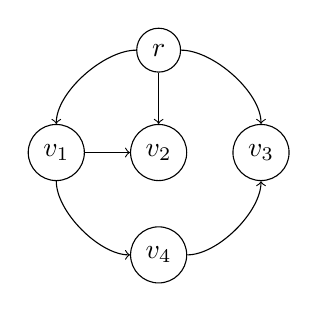
\begin{tikzpicture}[node distance={30mm}, main/.style = {draw, circle}] 
        \node[main] (r) at (0, 1.3) {$r$}; 
        \node[main] (1) at (-1.3, 0) {$v_1$};
        \node[main] (2) at (0, 0) {$v_2$};
        \node[main] (3) at (1.3, 0) {$v_3$};
        \node[main] (4) at (0, -1.3) {$v_4$};

        \draw[->] (r) to [out=180, in=90, looseness=0.75] (1);
        \draw[->] (r) -- (2);
        \draw[->] (r) to [out=0, in=90, looseness=0.75] (3);
        \draw[->] (1) -- (2);
        \draw[->] (1) to [out=270, in=180, looseness=0.75] (4);
        \draw[->] (4) to [out=0, in=270, looseness=0.75] (3);
    \end{tikzpicture} 
\end{center}
\vspace{-0.25cm}
Then the following two subgraphs are arborescences rooted at $r$.
\begin{center}
    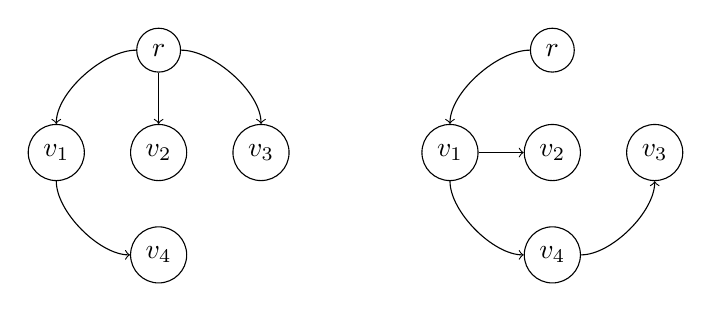
\begin{tikzpicture}[node distance={30mm}, main/.style = {draw, circle}] 
        \node[main] (r) at (0, 1.3) {$r$}; 
        \node[main] (1) at (-1.3, 0) {$v_1$};
        \node[main] (2) at (0, 0) {$v_2$};
        \node[main] (3) at (1.3, 0) {$v_3$};
        \node[main] (4) at (0, -1.3) {$v_4$};

        \node[main] (r') at (5, 1.3) {$r$}; 
        \node[main] (1') at (3.7, 0) {$v_1$};
        \node[main] (2') at (5, 0) {$v_2$};
        \node[main] (3') at (6.3, 0) {$v_3$};
        \node[main] (4') at (5, -1.3) {$v_4$};

        \draw[->] (r) to [out=180, in=90, looseness=0.75] (1);
        \draw[->] (r) -- (2);
        \draw[->] (r) to [out=0, in=90, looseness=0.75] (3);
        % \draw[->] (1) -- (2);
        \draw[->] (1) to [out=270, in=180, looseness=0.75] (4);
        % \draw[->] (4) to [out=0, in=270, looseness=0.75] (3);

        \draw[->] (r') to [out=180, in=90, looseness=0.75] (1');
        % \draw[->] (r') -- (2');
        % \draw[->] (r') to [out=0, in=90, looseness=0.75] (3');
        \draw[->] (1') -- (2');
        \draw[->] (1') to [out=270, in=180, looseness=0.75] (4');
        \draw[->] (4') to [out=0, in=270, looseness=0.75] (3');
    \end{tikzpicture} 
\end{center}
\vspace{-0.25cm}
On the other hand, the following two subgraphs are not arborescences
rooted at $r$: the first one is not a tree, and the second has no directed 
path from $r$ to $v_4$.
\begin{center}
    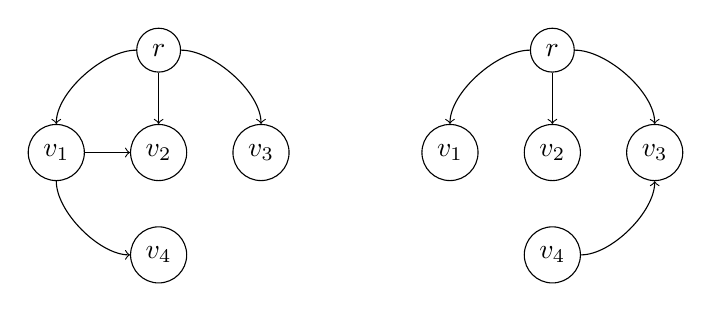
\begin{tikzpicture}[node distance={30mm}, main/.style = {draw, circle}] 
        \node[main] (r) at (0, 1.3) {$r$}; 
        \node[main] (1) at (-1.3, 0) {$v_1$};
        \node[main] (2) at (0, 0) {$v_2$};
        \node[main] (3) at (1.3, 0) {$v_3$};
        \node[main] (4) at (0, -1.3) {$v_4$};

        \node[main] (r') at (5, 1.3) {$r$}; 
        \node[main] (1') at (3.7, 0) {$v_1$};
        \node[main] (2') at (5, 0) {$v_2$};
        \node[main] (3') at (6.3, 0) {$v_3$};
        \node[main] (4') at (5, -1.3) {$v_4$};

        \draw[->] (r) to [out=180, in=90, looseness=0.75] (1);
        \draw[->] (r) -- (2);
        \draw[->] (r) to [out=0, in=90, looseness=0.75] (3);
        \draw[->] (1) -- (2);
        \draw[->] (1) to [out=270, in=180, looseness=0.75] (4);
        % \draw[->] (4) to [out=0, in=270, looseness=0.75] (3);

        \draw[->] (r') to [out=180, in=90, looseness=0.75] (1');
        \draw[->] (r') -- (2');
        \draw[->] (r') to [out=0, in=90, looseness=0.75] (3');
        % \draw[->] (1') -- (2');
        % \draw[->] (1') to [out=270, in=180, looseness=0.75] (4');
        \draw[->] (4') to [out=0, in=270, looseness=0.75] (3');
    \end{tikzpicture} 
\end{center}
\vspace{-0.25cm}
The following theorem gives us a useful characterization of arborescences.

\begin{theo}[Characterization of Arborescences]{theo:3.1}
    Let $G = (V, E)$ be a connected graph and let $T = (V, F)$ be a subgraph. 
    Then $T$ is an arborescence rooted at $r$ if and only if both 
    of the following conditions hold:
    \begin{enumerate}[(1)]
        \item every $v \in V$ with $v \neq r$ has exactly one incoming edge in $T$; and 
        \item $T$ has no directed cycles. 
    \end{enumerate}
\end{theo}
\begin{pf}[Theorem~\ref{theo:3.1}]
    $(\Rightarrow)$ First, we check that condition (1) holds. Consider a vertex 
    $v \in V$ with $v \neq r$. Since undirected $T$ is a spanning tree, 
    there is a unique (simple) path from $r$ to $v$ in undirected $T$. 
    The last edge on this path is incoming for $v$. Hence, all other edges 
    incident to $v$ in undirected $T$ should be outgoing edges for $v$ 
    (because the neighbours of $v$ also have unique simple paths from $v$ 
    to them in undirected $T$). This proves (1). To see that condition (2) 
    holds, note that undirected $T$ is acyclic as it is a spanning tree, 
    so it could not possibly have any directed cycles either. 

    $(\Leftarrow)$ Suppose that $V = (T, F)$ satisfies conditions (1) and (2). 
    First, we show that for all $v \in V$ with $v \neq r$, there exists 
    a directed path from $r$ to $v$ in $T$, which is condition (ii) of the 
    definition of an arborescence. Let $(v_1, v)$ be the unique edge 
    incoming to $v$ by condition (1), let $(v_2, v_1)$ be the unique edge 
    incoming to $v_1$, and so on. By contradiction, suppose that we 
    cannot reach $r$ by backtracking in this way. Then at some point, 
    we must visit the same node at least twice because $G$ is a finite graph. 
    But this creates a directed cycle, contradicting condition (2). Thus, 
    there is a directed path from $r$ to $v$ in $T$. 

    Now, we verify condition (i) that undirected $T$ is a spanning tree. 
    Note that we can get from $r$ to any other vertex $v$, so 
    undirected $T$ is connected. Moreover, $r$ has no incoming edges 
    because if $(v, r)$ is an incoming edge, then the directed path from 
    $r$ to $v$ followed by $(v, r)$ forms a directed cycle, contradicting 
    condition (2). Since every edge is incoming for exactly one of its 
    endpoints, the total number of edges in $T$ is 
    \[ \sum_{u=r} 0 + \sum_{\substack{u\in V \\ u\neq r}} 1 = |V| - 1. \] 
    By the fundamental theorem of trees (Theorem~\ref{theo:2.1}), 
    it follows that undirected $T$ is a spanning tree. \qed 
\end{pf}

\subsection{Minimum Cost Arborescences}\label{subsec:3.2}
Given a directed graph $G = (V, E)$, a distinguished node $r$, and edge 
costs $c_e \geq 0$ for each $e \in E$, our goal is to find an arborescence
rooted at $r$ so that the total edge cost is minimized. 

Let's try to transfer our knowledge from the minimum spanning tree problem. 
Do the analogues of the cycle and cut properties hold for arborescences?
It turns out we can find a counterexample to both in the same graph. 
Consider the following graph $G = (V, E)$ with associated edge costs. 
\begin{center}
    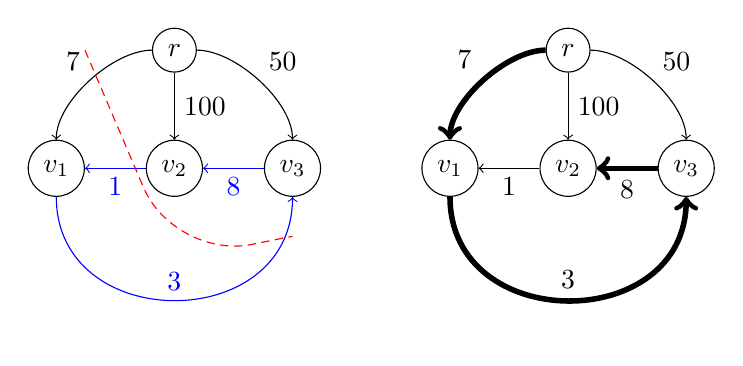
\begin{tikzpicture}[
        node distance={30mm}, 
        main/.style = {draw, circle},
        xs/.style = {xshift=#1 mm},
        ys/.style = {yshift=#1 mm}
    ] 
        \node[main] (r) at (0, 1.5) {$r$}; 
        \node[main] (1) at (-1.5, 0) {$v_1$};
        \node[main] (2) at (0, 0) {$v_2$};
        \node[main] (3) at (1.5, 0) {$v_3$};

        \node[main] (r') at (5, 1.5) {$r$}; 
        \node[main] (1') at (3.5, 0) {$v_1$};
        \node[main] (2') at (5, 0) {$v_2$};
        \node[main] (3') at (6.5, 0) {$v_3$};

        \draw[->] (r) to [out=180, in=90, looseness=0.75] node[midway, above left] {7} (1);
        \draw[->] (r) -- node[midway, right] {100} (2);
        \draw[->] (r) to [out=0, in=90, looseness=0.75] node[midway, above right] {50} (3);
        \draw[->, color=blue] (2) -- node[midway, below] {1} (1);
        \draw[->, color=blue] (3) -- node[midway, below] {8} (2);
        \draw[->, color=blue] (1) to [out=270, in=270, looseness=1.5] node[midway, above] {3} (3);

        \draw[rounded corners=10mm, red, densely dashed] 
            ([xs=-8.5] r.west) -- ([ys=-8] 2.south) -- ([ys=-5] 3.south);

        \draw[->, line width=2pt] (r') to [out=180, in=90, looseness=0.75] node[midway, above left] {7} (1');
        \draw[->] (r') -- node[midway, right] {100} (2');
        \draw[->] (r') to [out=0, in=90, looseness=0.75] node[midway, above right] {50} (3');
        \draw[->] (2') -- node[midway, below] {1} (1');
        \draw[->, line width=2pt] (3') -- node[midway, below] {8} (2');
        \draw[->, line width=2pt] (1') to [out=270, in=270, looseness=1.5] node[midway, above] {3} (3');
    \end{tikzpicture} 
\end{center}
\vspace{-0.25cm}
The minimum cost arborescence is given to the right with cost 
$7 + 3 + 8 = 18$. Consider the cut (in red) and cycle (in blue) above. 
Then the cut property fails to hold because the edge $(v_2, v_1)$ of cost $1$ was 
not picked in a minimum cost arborescence, and the cycle property fails 
to hold because the edge $(v_3, v_2)$ of maximum cost $8$ in the cycle 
was picked in a minimum cost arborescence. 

Can we instead consider the union of minimum cost incoming edges 
(vertex by vertex), excluding the root $r$? For the above example, 
if we start with $v_1$, we'd pick $(v_2, v_1)$ as it is the minimum cost 
edge incoming to $v_1$. Then $(v_1, v_3)$ is the minimum cost edge 
incoming to $v_3$ and $(v_3, v_2)$ is the minimum cost edge incoming to 
$v_2$. This yields the same directed cycle highlighted in blue above!

So this strategy does not immediately work. But if the strategy 
did happen to give us an arborescence, then we are already done! 
All we need to do is tweak it slightly. The idea is to compute 
\[ y_v = \min_{(u,v)\in E} c_{(u, v)} \] 
for all vertices $v \in V$ with $v \neq r$. In particular, any edge using this 
vertex needs to pay this cost anyways. Then for all $(u, v) \in E$, we can 
define new edge costs 
\[ c'_{(u, v)} = c_{(u, v)} - y_v. \] 
We give the edge costs $c'_e$ (in blue) and the values $y_v$ (in purple) for the above example.
Notice that some of the edges turn out to be free.
\begin{center}
    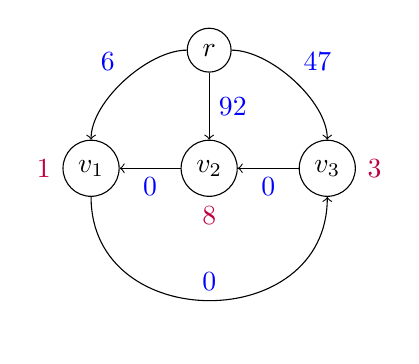
\begin{tikzpicture}[
        node distance={30mm}, 
        main/.style = {draw, circle},
    ] 
        \node[main] (r) at (0, 1.5) {$r$}; 
        \node[main] (1) at (-1.5, 0) {$v_1$};
        \node[color=purple] (1cost) at (-2.1, 0) {$1$};
        \node[main] (2) at (0, 0) {$v_2$};
        \node[color=purple] (2cost) at (0, -0.6) {$8$};
        \node[main] (3) at (1.5, 0) {$v_3$};
        \node[color=purple] (3cost) at (2.1, 0) {$3$};

        \draw[->] (r) to [out=180, in=90, looseness=0.75] node[midway, above left, text=blue] {6} (1);
        \draw[->] (r) -- node[midway, right, text=blue] {92} (2);
        \draw[->] (r) to [out=0, in=90, looseness=0.75] node[midway, above right, text=blue] {47} (3);
        \draw[->] (2) -- node[midway, below, text=blue] {0} (1);
        \draw[->] (3) -- node[midway, below, text=blue] {0} (2);
        \draw[->] (1) to [out=270, in=270, looseness=1.5] node[midway, above, text=blue] {0} (3);
    \end{tikzpicture} 
\end{center}
\vspace{-0.25cm}
